\documentclass{article}

\usepackage{float}
\usepackage{xcolor}
\usepackage{parskip}
\usepackage{eulervm}
\usepackage{graphicx}
\usepackage{setspace}
\usepackage{geometry}
\usepackage{microtype}
\usepackage[T1]{fontenc}
\usepackage[utf8]{inputenc}
\usepackage{amsfonts, amsmath, amssymb}

\setstretch{1.50}
\geometry{paper=letterpaper, layout=letterpaper, margin=1in}

\begin{document}

\begin{titlepage}
    \begin{center}
        \vspace*{2cm}
        {\Huge \textbf{ ME 4638: Computational Mechanics Lab}} \\
        \vspace{1cm}
        {\Large \textbf{Assignment III}} \\

        \vfill

        \textit{\large Submitted by:} \\
        \vspace{0.3cm}
        \textbf{Abdullah al Azmi, 220011230} \\
        % \textbf{Std. ID: 220011230} \\

        \vfill

        \textit{\large Submitted to:} \\
        \vspace{0.3cm}
        \textbf{\Large Sefat Mahmud Siddique} \\
        \textbf{Junior Lecturer, Department of Mechanical and Production Engineering} \\

        \vfill

        \textbf{Date of Submission: \today}
        \vspace*{1cm}
    \end{center}
\end{titlepage}

\newpage

\section*{Problem I}

\subsection*{Reynolds number: 2000}

\subsubsection*{Velocity Contour}

\begin{figure}[H]
    \centering
    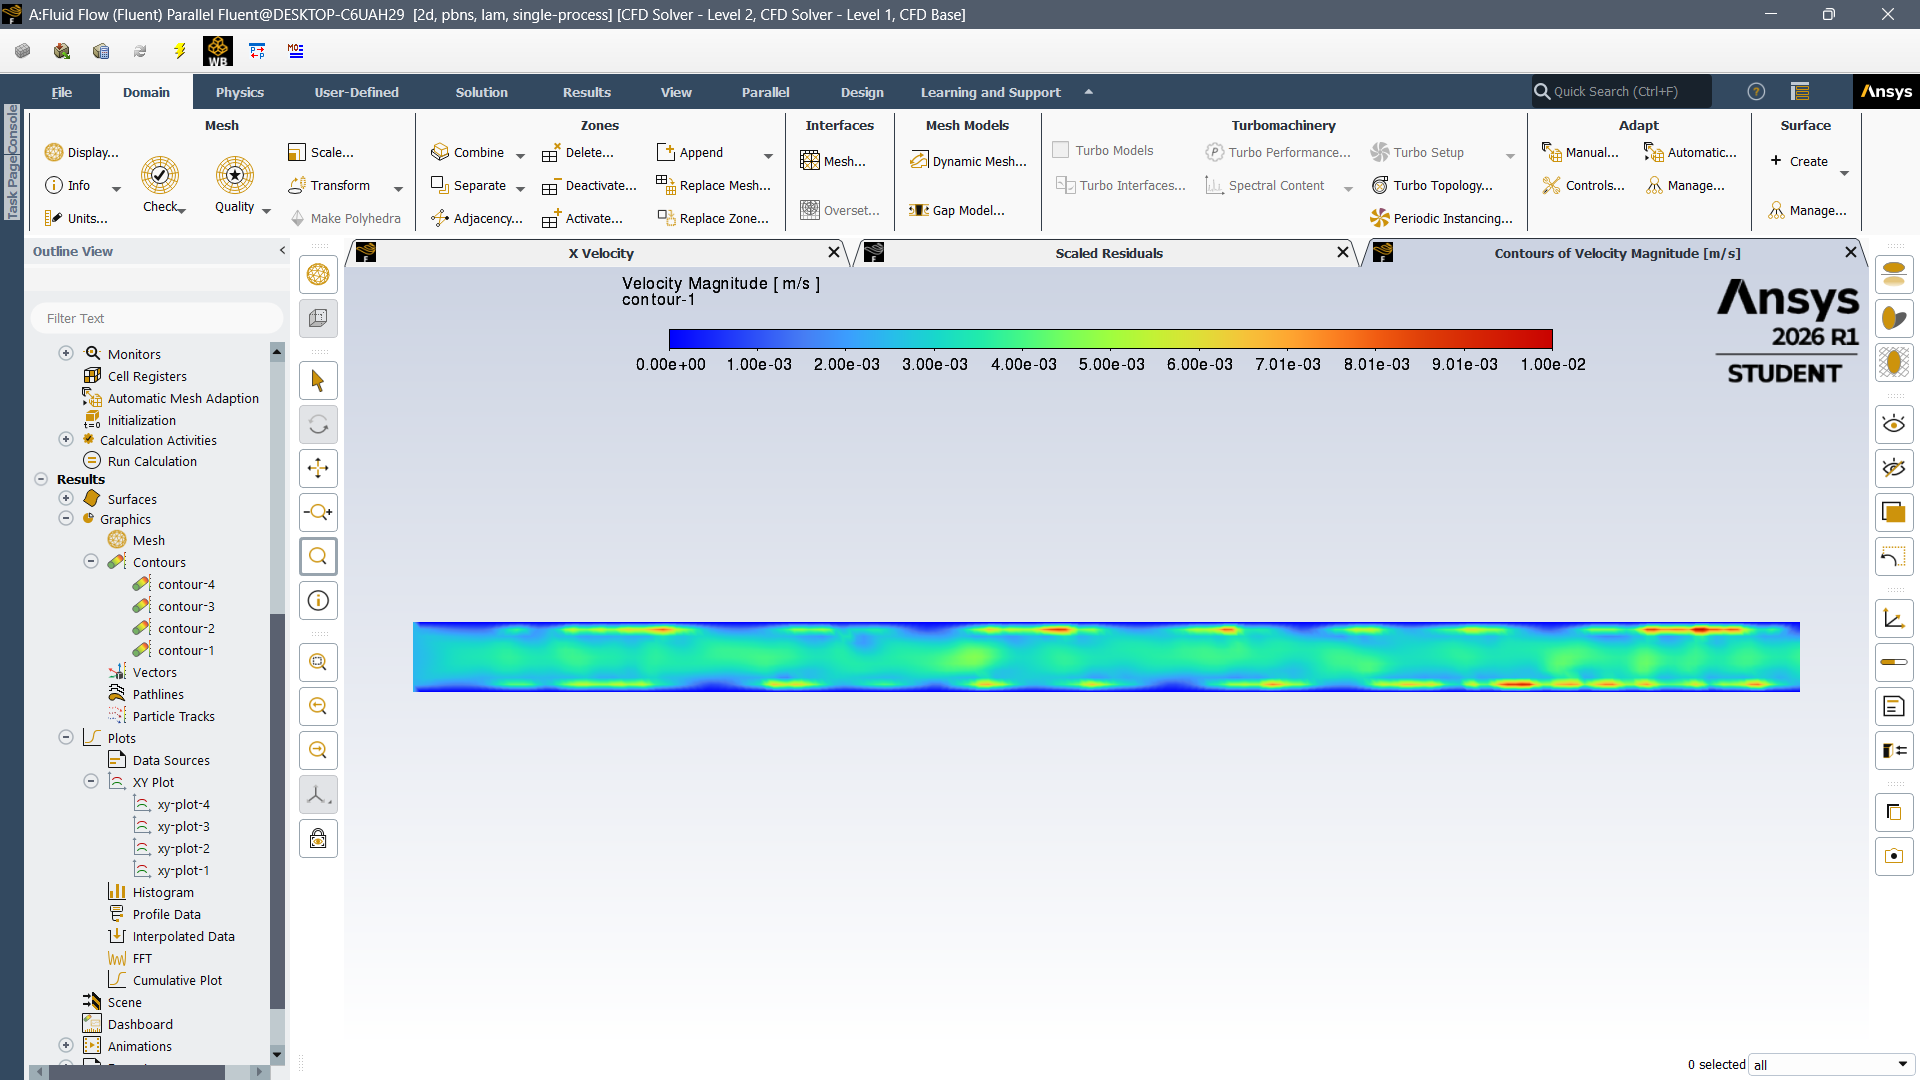
\includegraphics[width=0.85\textwidth]{images/Screenshot 2026-07-24 111336.png}
\end{figure}

\subsubsection*{Pressure Contour}

\begin{figure}[H]
    \centering
    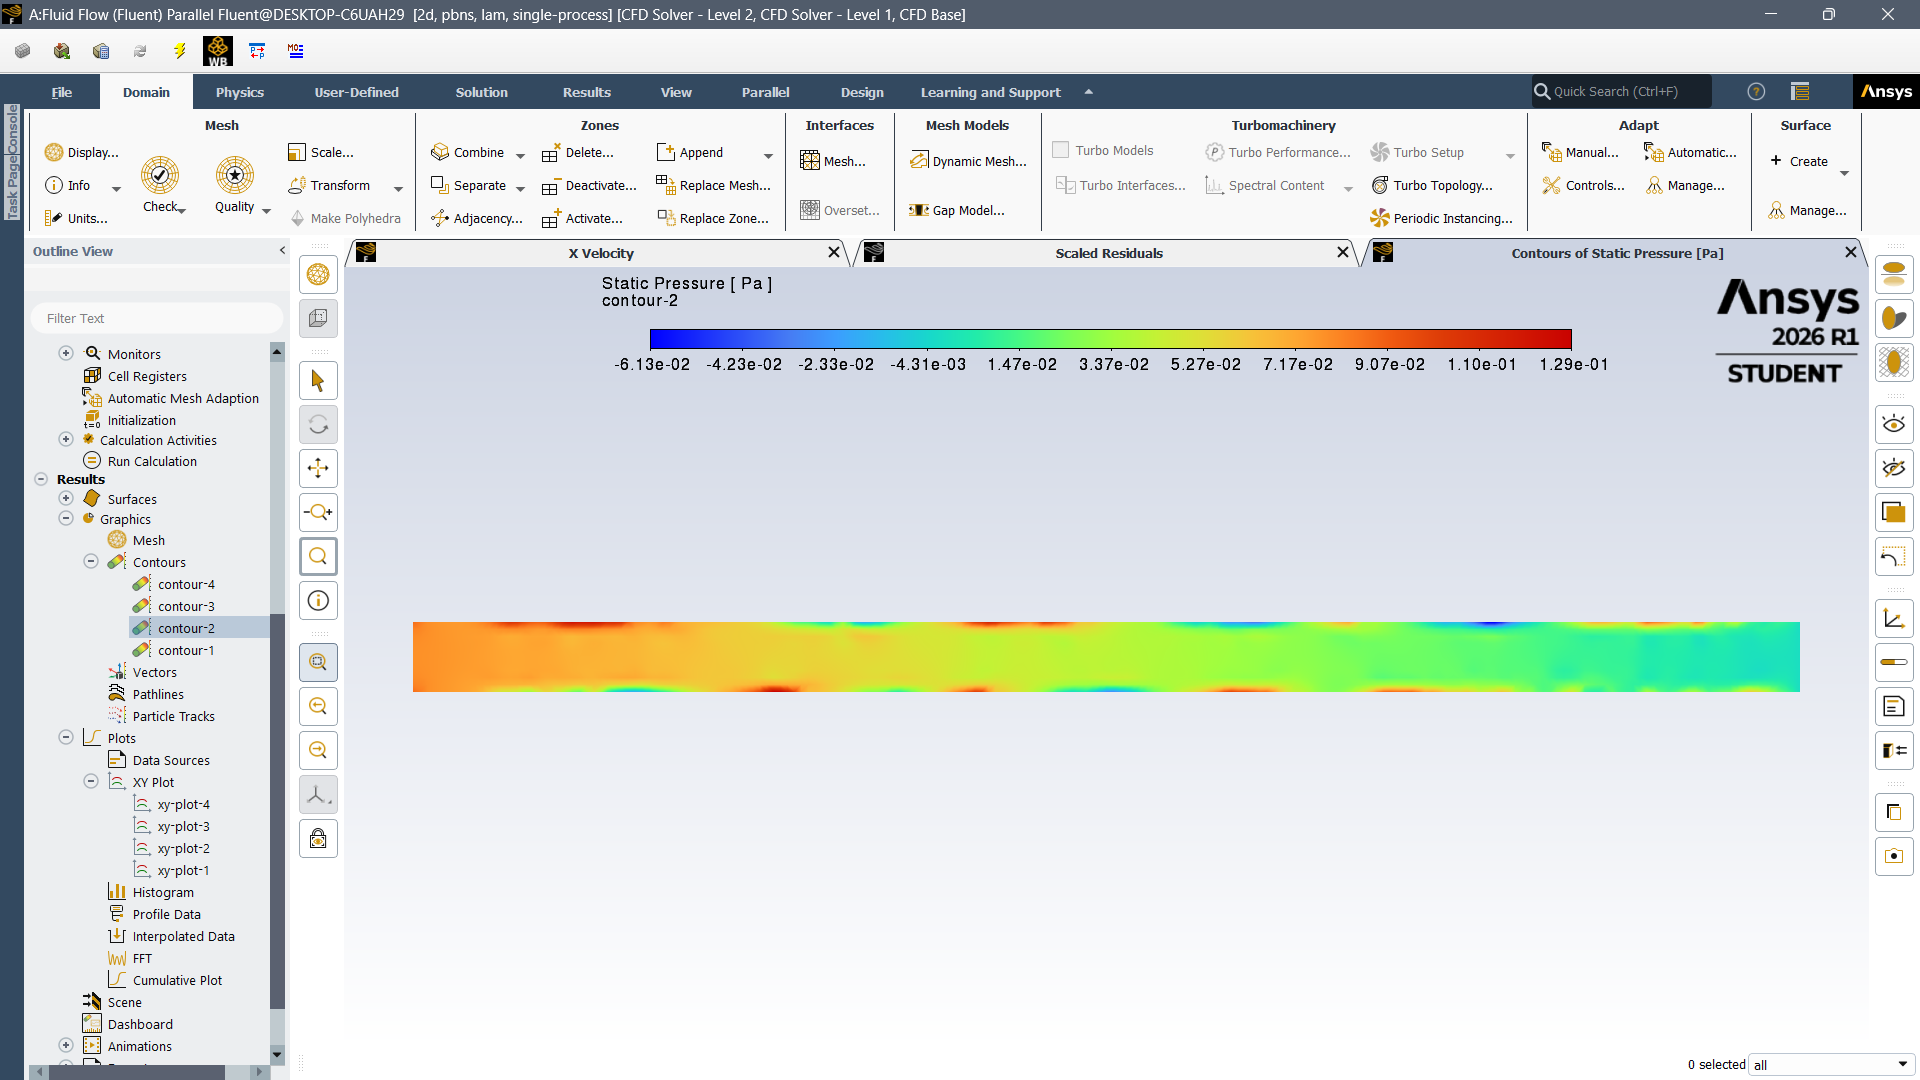
\includegraphics[width=0.85\textwidth]{images/Screenshot 2026-07-24 111350.png}
\end{figure}

\subsubsection*{Velocity Boundary Layer Curve at L=100 mm}

\begin{figure}[H]
    \centering
    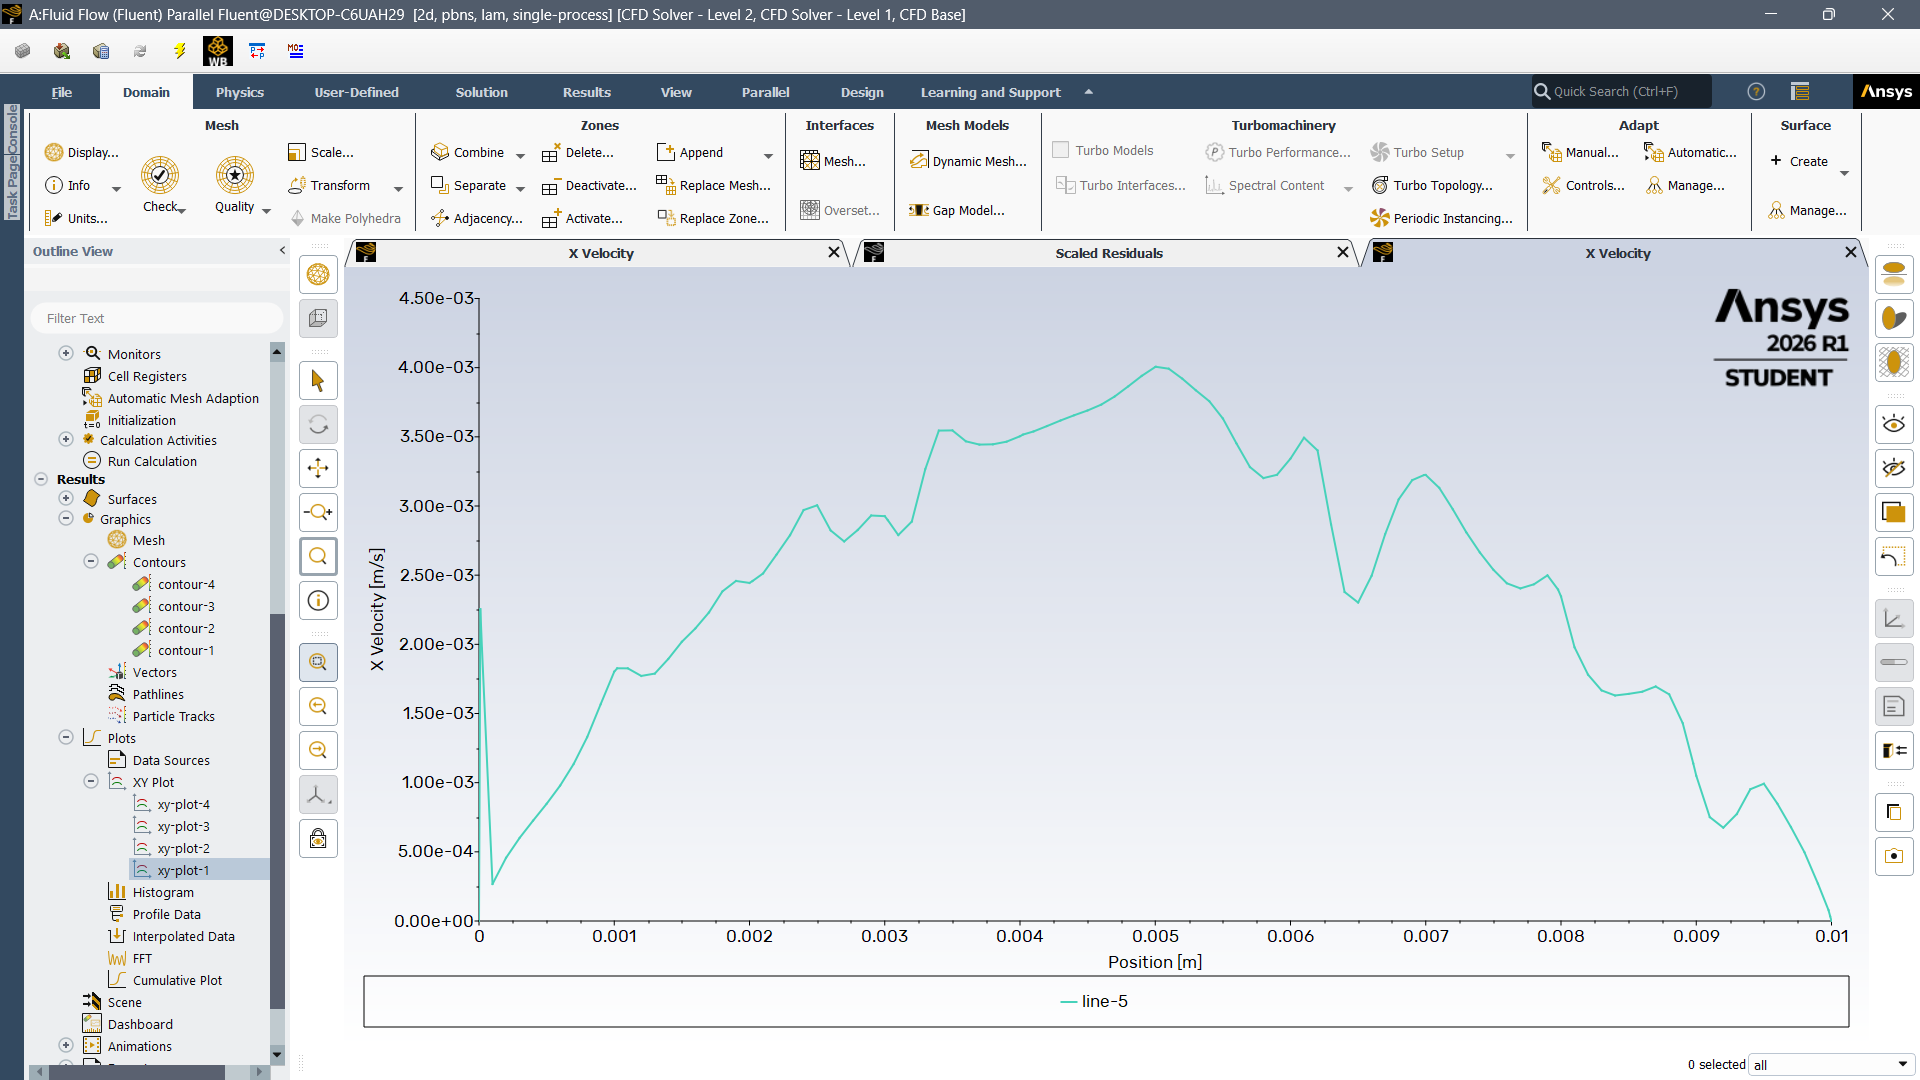
\includegraphics[width=0.85\textwidth]{images/Screenshot 2026-07-24 111437.png}
\end{figure}

\subsubsection*{Velocity Boundary Layer Curve at L=180 mm}

\begin{figure}[H]
    \centering
    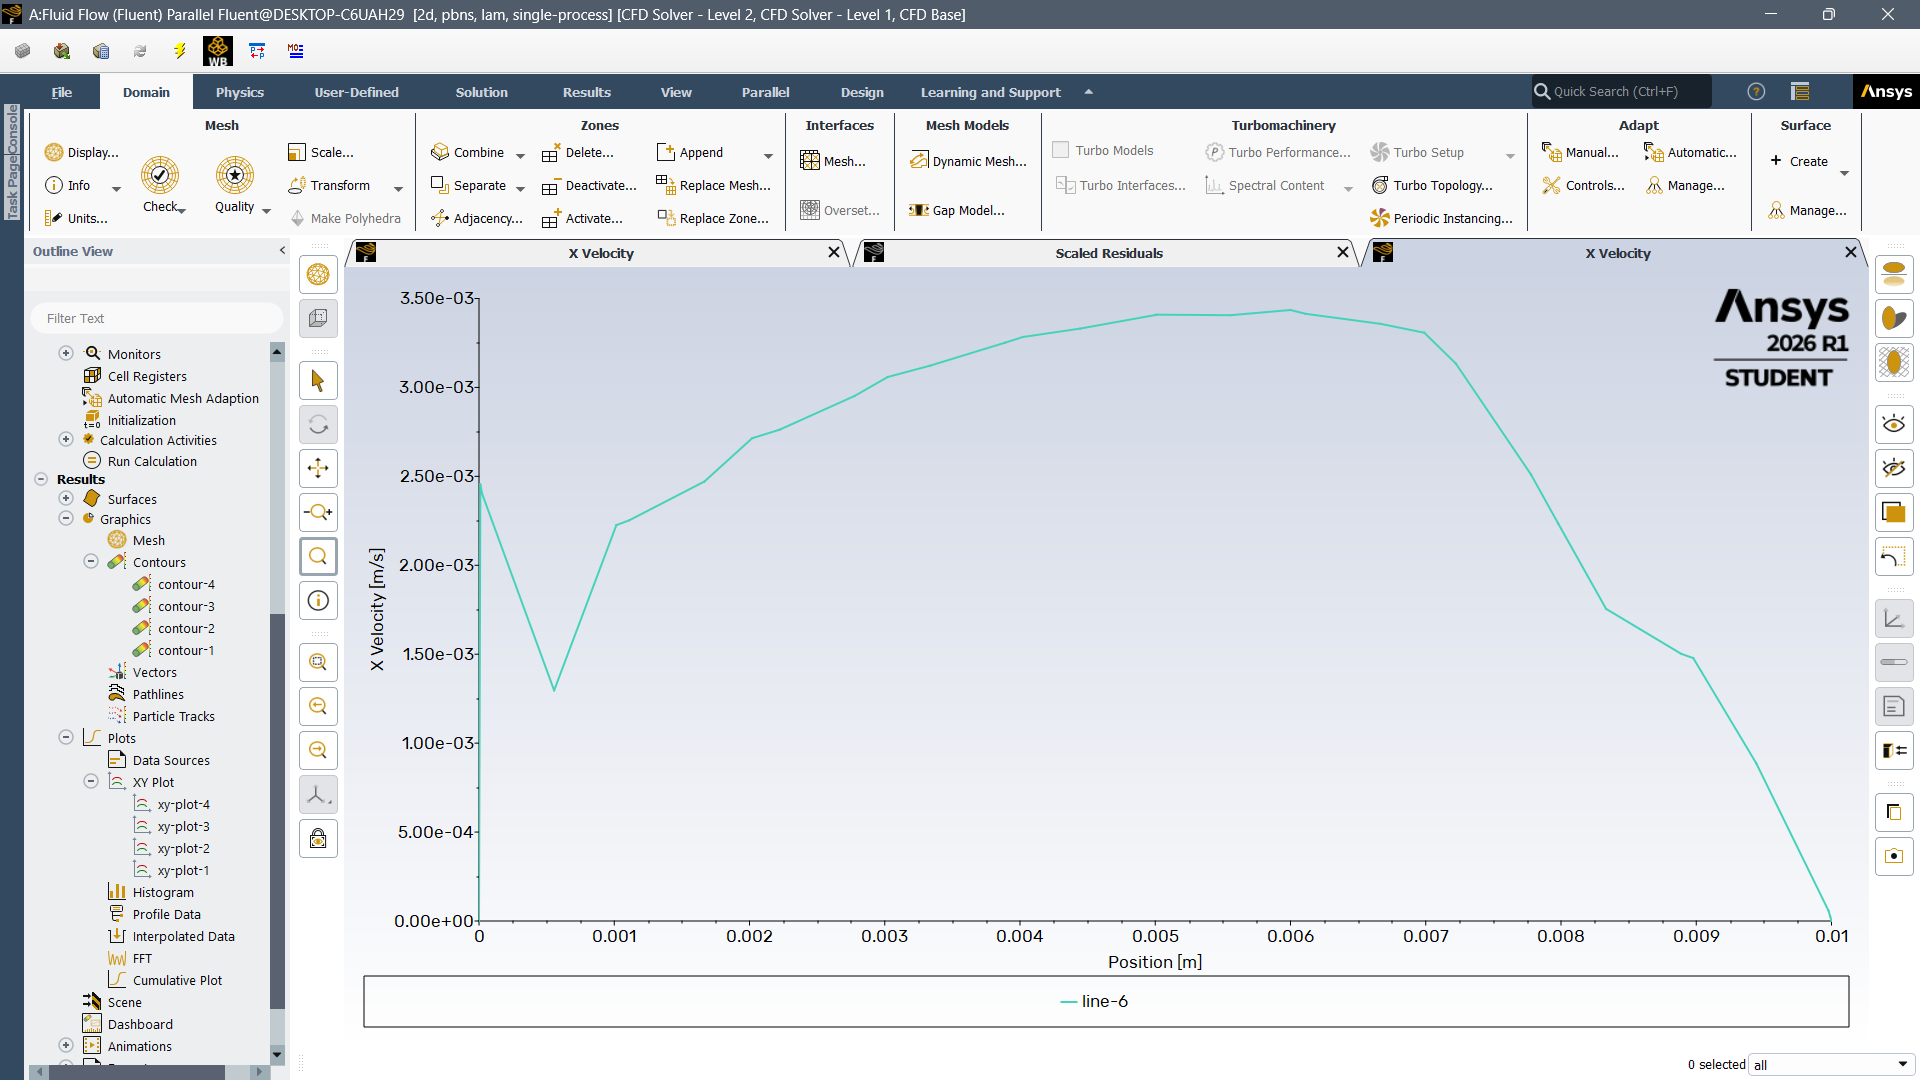
\includegraphics[width=0.85\textwidth]{images/Screenshot 2026-07-24 111450.png}
\end{figure}

\subsection*{Reynolds number: 2500}

\subsubsection*{Velocity Contour}

\begin{figure}[H]
    \centering
    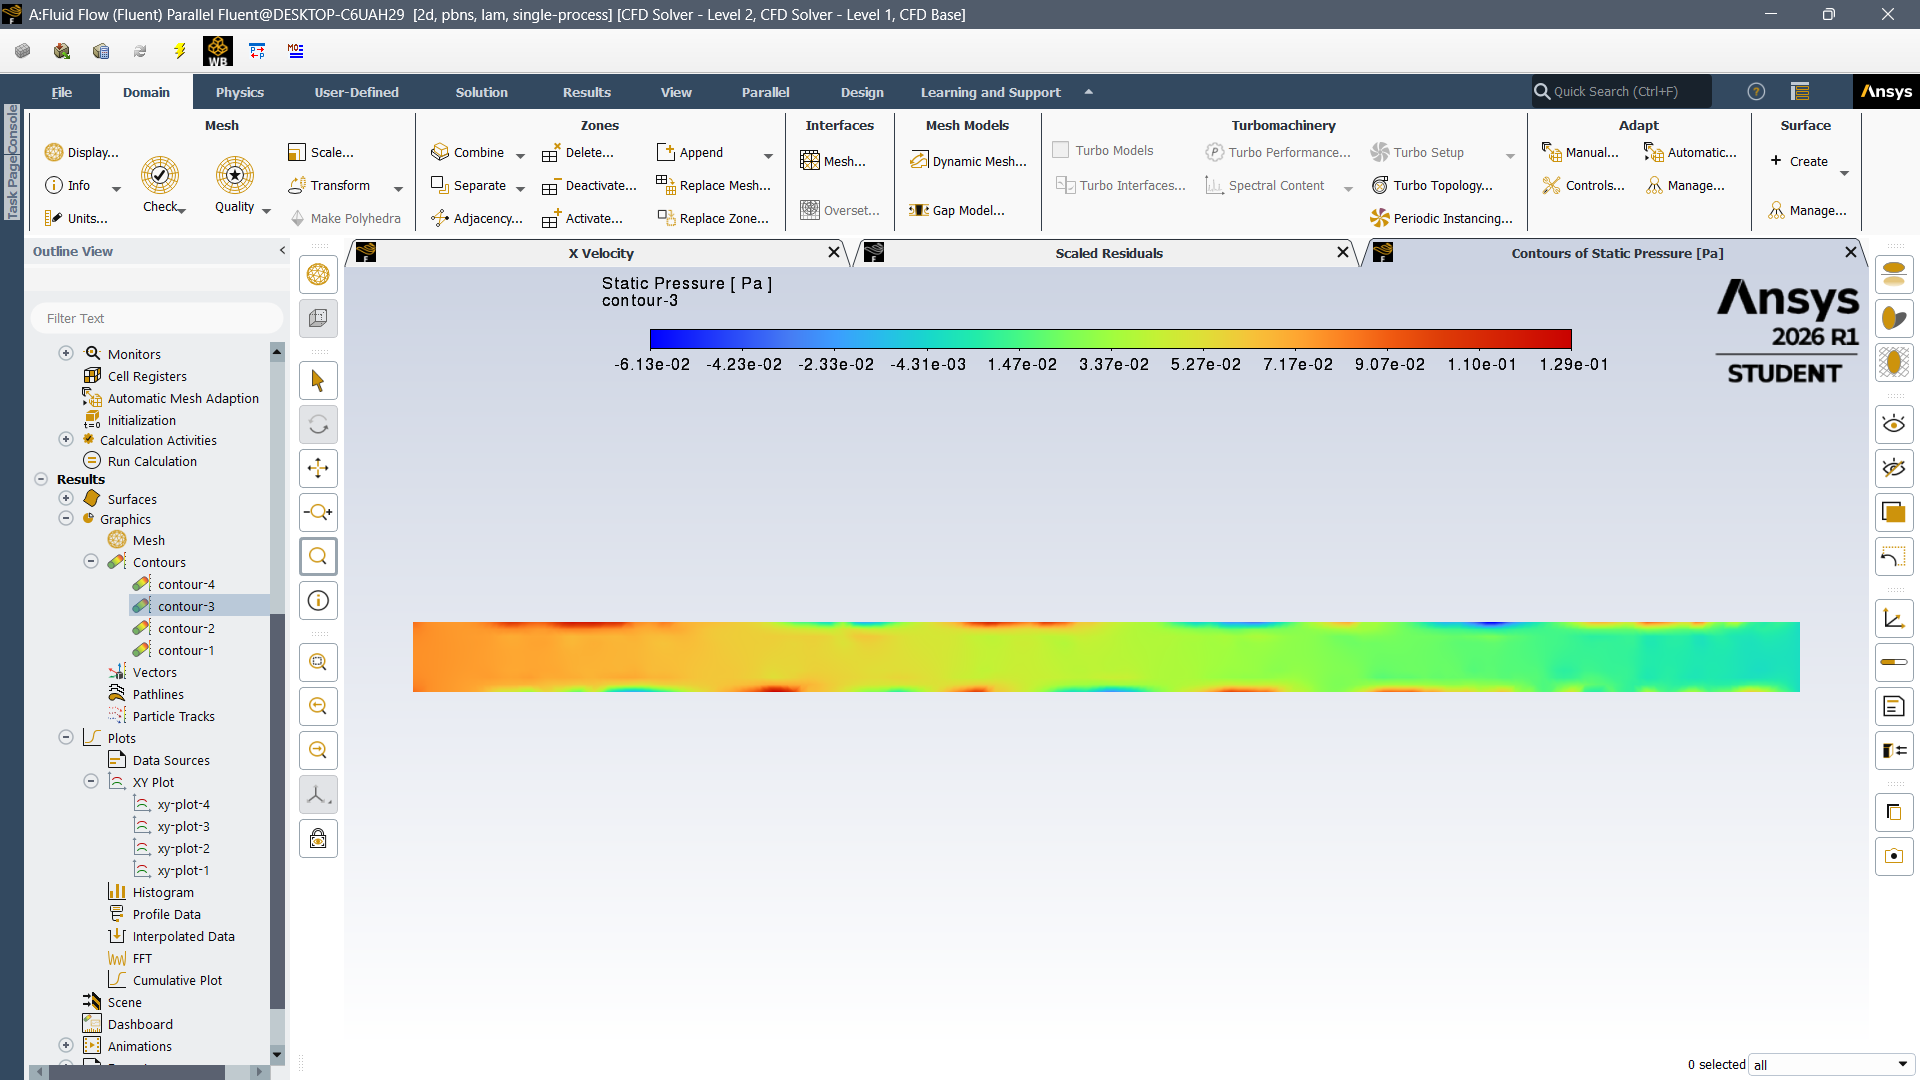
\includegraphics[width=0.85\textwidth]{images/Screenshot 2026-07-24 111402.png}
\end{figure}

\subsubsection*{Pressure Contour}

\begin{figure}[H]
    \centering
    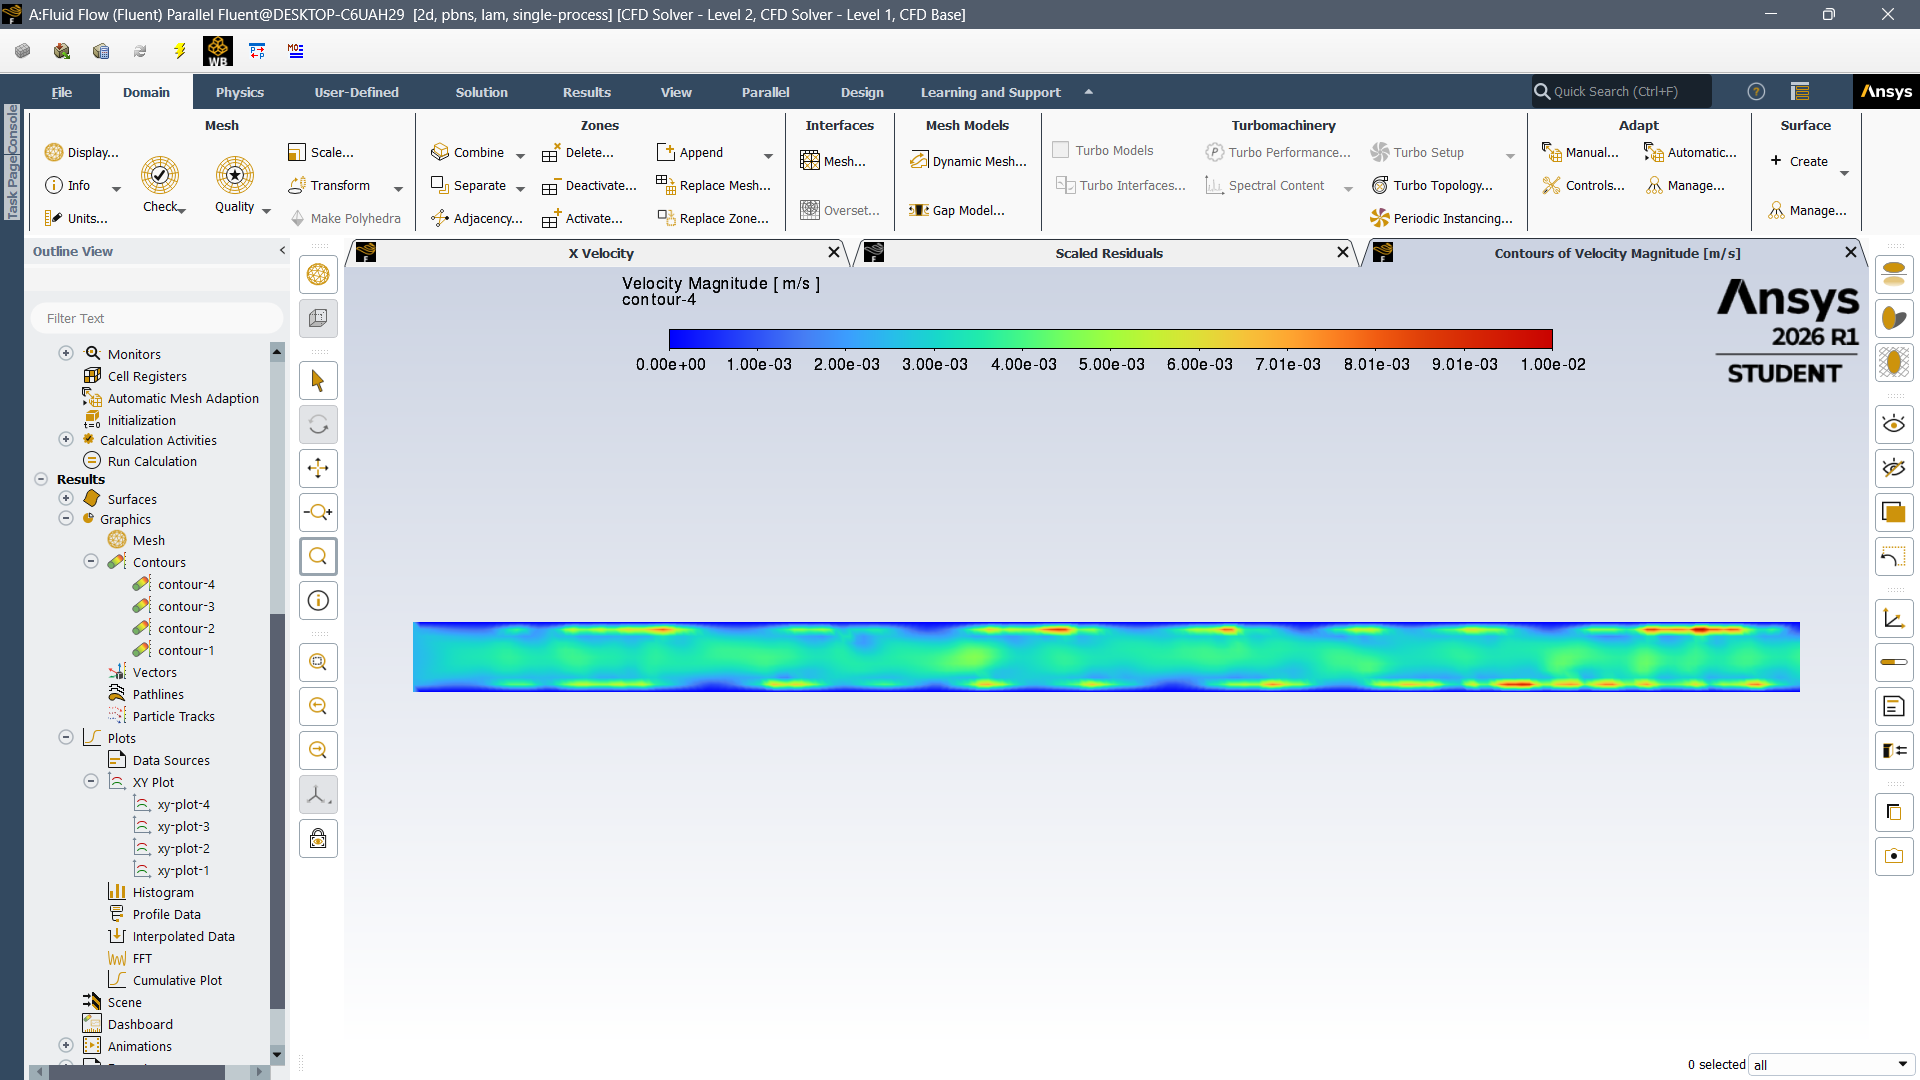
\includegraphics[width=0.85\textwidth]{images/Screenshot 2026-07-24 111414.png}
\end{figure}

\subsubsection*{Velocity Boundary Layer Curve at L=100 mm}

\begin{figure}[H]
    \centering
    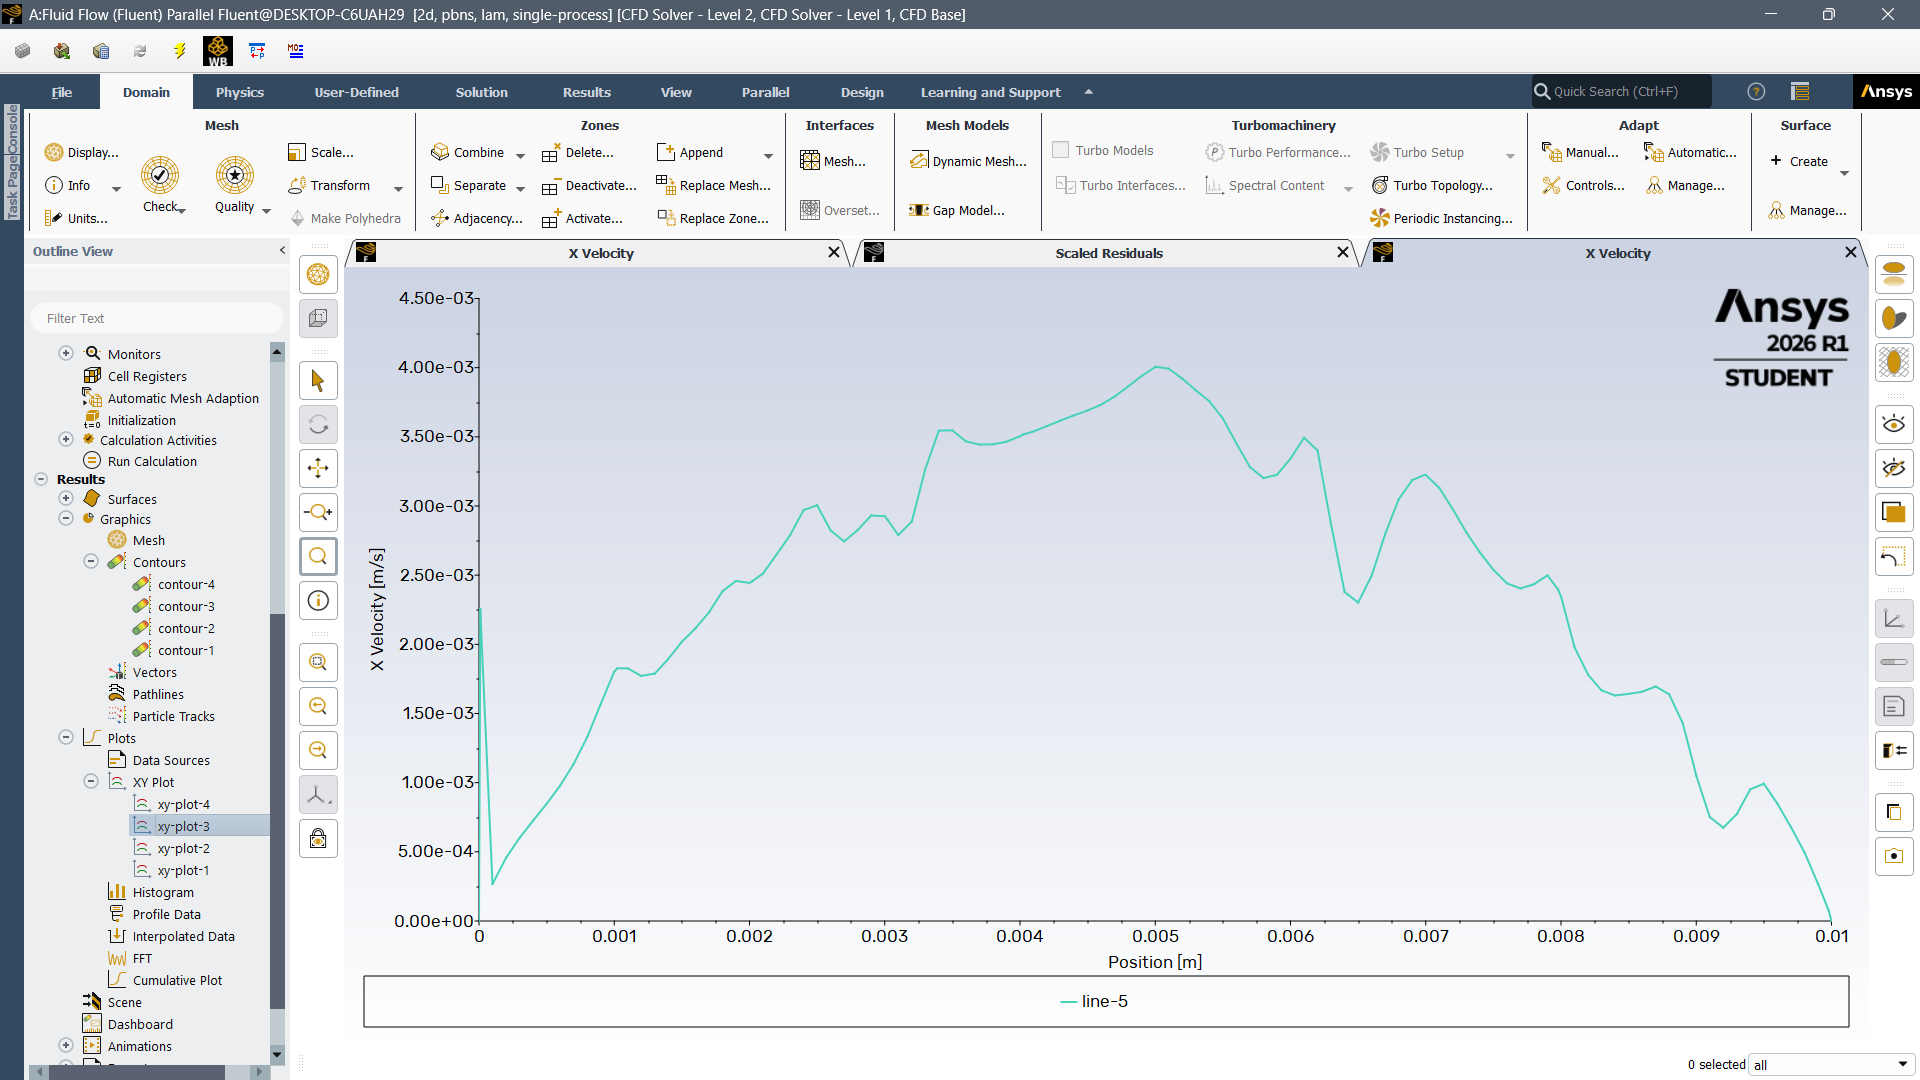
\includegraphics[width=0.85\textwidth]{images/Screenshot 2026-07-24 111502.png}
\end{figure}

\subsubsection*{Velocity Boundary Layer Curve at L=180 mm}

\begin{figure}[H]
    \centering
    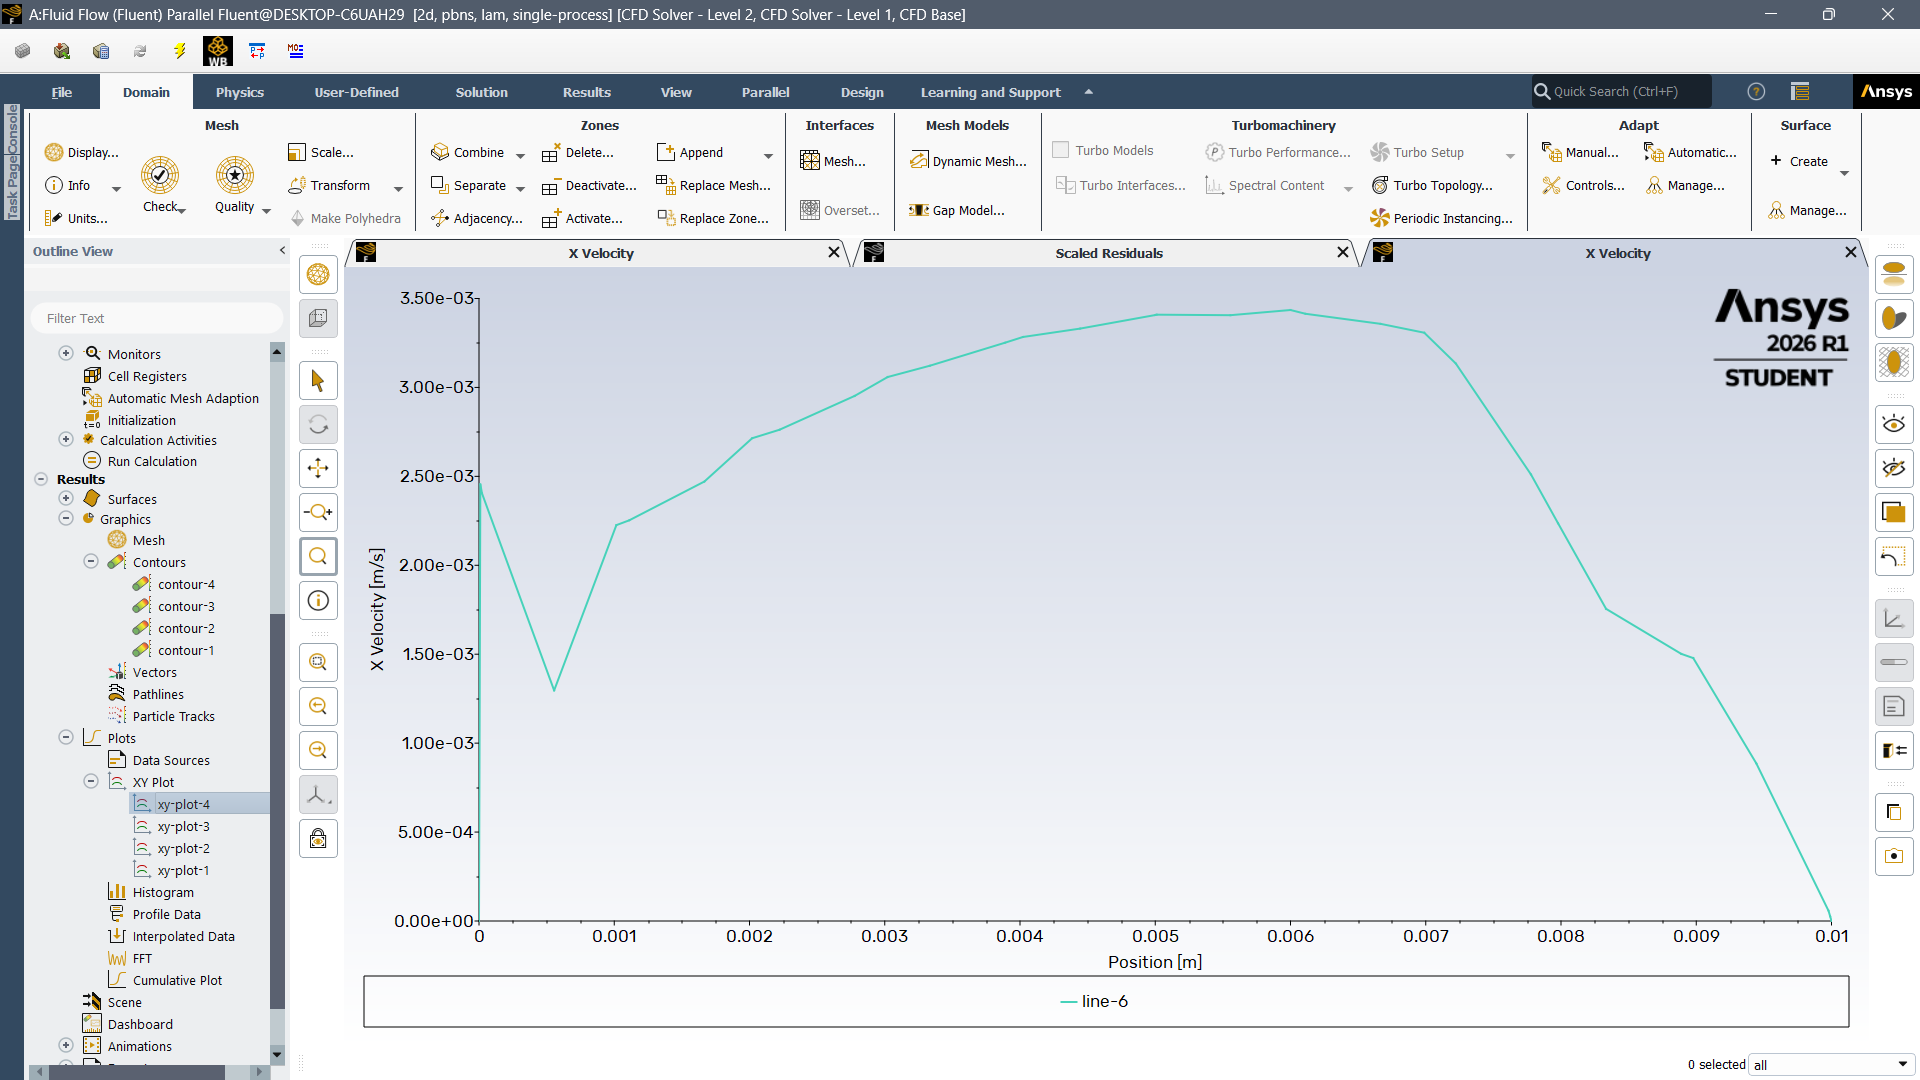
\includegraphics[width=0.85\textwidth]{images/Screenshot 2026-07-24 111515.png}
\end{figure}

\end{document}